\subsection{The Turing machine $M_\text{subword}$}

This Turing machine should recognize the language
$$
    L_\text{subword} = \left\{ w_1 \# w_2 \mid \text{$w_1 \in \{0,1\}^*$ and $w_2$ is a substring of $w_1$} \right\}.
$$


\subsubsection{Description}

\paragraph{High-level description}

Repeatedly, we compare the first word to the second. If the first word starts with the second, accept. Otherwise, mark off the first unmarked letter from the first word and repeat. If the first word is completely marked off, reject. 


\paragraph{Implementation-level description}
$M_{\text{subword}}=$
``on input $w \in \{0,1,\#\}^*$:
\begin{enumerate}
    \item Read the current cell, remember its value as $c$, and write $\$$ to it. \\
        If $c=\#$, move right one cell and accept if that cell's value is $\_$, reject otherwise.
    \item Move right until $\#$, then move right while reading $X$s and $Y$s.
    \item If the current cell has the same value as $c$, write $X$ if $C=2$ or $Y$ if $c=1$ to the current cell and move left until encountering either $\$$, $X$, or $Y$. \\
        Otherwise, if the current cell's value is $\_$, accept. \\
        Otherwise, go to step 5.
    \item Move right one cell. Read this cell's value, remember it as $c$, and write $Y$ to it. Go to step 2.
    \item Move left until reading $\$$. While moving left, replace all $X$ with $0$ and $Y$ with $1$.
    \item Move right one cell and go to step 1."
\end{enumerate}

\subsubsection{Theoretical analysis of complexity}

The word $x_n$ that will require the highest number of transitions for a particular $n>2$ is of the form $x_n=1^{n-3} \# 1 0$. Note that the word $0^{n-3} \#  0 1$ would be equivalent in respect to the fact that it will require the same number of steps, but we will look at $x_n$.

On input $x_n=1^{n-3} \# 1 0$ for $n>2$ (as seen in the example screenshot to the right where $n=3$):
\begin{enumerate}
    \item Let $i$ denote the number of letters marked off the first word. Initially, $i=1$. Mark off the next letter of the first word and move to the beginning of the second word ($n-i-1$ transitions).
    \item Mark off the first letter of the second word and move left until reading the marked character of the first word ($n-i-1$ transitions). 
    \item Read the cell to the right and compare that to the second letter of the second word ($n-i$ transitions).
    \item Move back to the beginning (because the letters did not match) ($n-i$ transitions)
    \item Move one cell to the right ($1$ transition). If $i \leq n-1$, go to step 1.
    \item Now only 7 transitions remain, after which the word is rejected.
\end{enumerate}

Counting the number of transitions we obtain
\begin{align*}
    f(n)
        &= \sum_{i=1}^{n-1}(n-i-1+n-i-1+n-i+n-i+1) + 7 \\
        &= \sum_{i=1}^{n-1}(4n -4i-1) + 7 \\
        &= \frac{n-1}{2}(4n-4-1+4n-4(n-1)-1) + 7 \\
        &= \frac{n-1}{2}(4n-2) + 7 \\
        &= (n-1)(2n-1)+7 \\
        &= 2n^2 - 3n + 6
\end{align*}
for $n>2$. 

Manual testing showed that $f(0)=0$, $f(1)=1$, and $f(2)=2$, so we can use $f(n)$ for all $n$ and be convinced that for any $n$, the value of $f(n)$ will be greater or equal to the number of transitions required. Hence
$$ M_\text{subword} \in \text{DTIME}(2n^2 - 3n + 6), $$
and so its complexity is in the order of $\mathcal{O}(n^2)$.

\subsubsection{Practical analysis of complexity}

The theoretical results are evident in practical trials. The data collected in \code{data/subword-ones.csv} confirms the findings of $f$ (the values were cross-checked). Furthermore, the plot below shows how this worst-case scenario behaves as a plot of $n$ against the number of transitions made by the machine. 

\begin{center}
    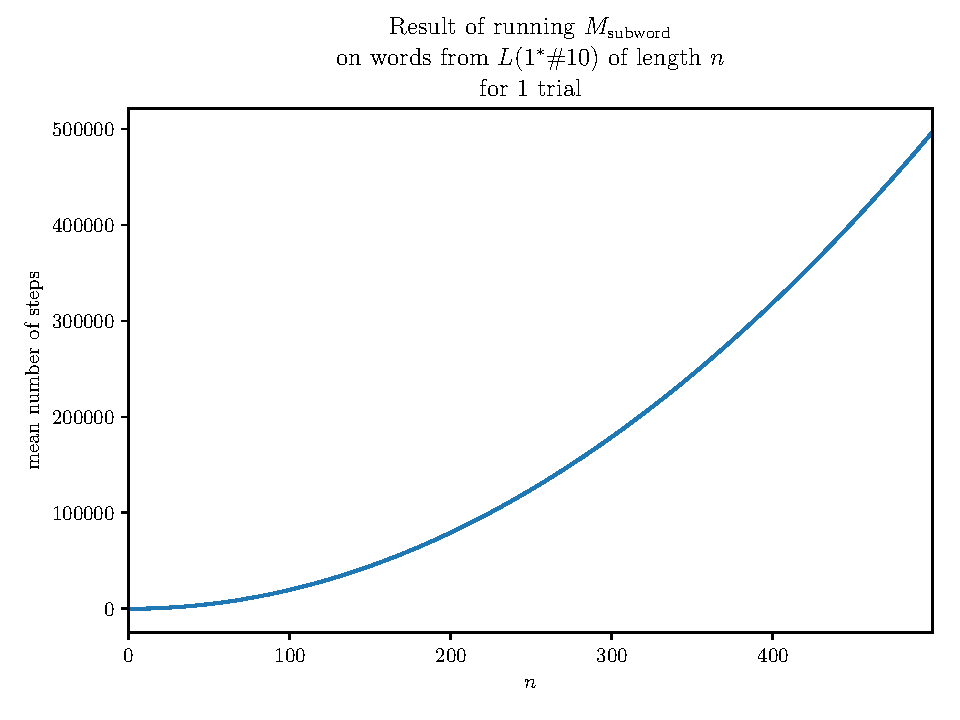
\includegraphics[width=\textwidth]{images/plots/subword-ones.pdf}
\end{center}

Other types of input words were also tested; please refer to the plots in section \ref{plots_subword}, as well as the CSV data in \code{data/subword-*.csv}. 

\subsubsection{An improvement: $M_\text{subword\_fast}$}

Upon looking at the findings, another Turing machine, $M_\text{subword\_fast}$ was created that would be more optimal. Instead of only verifying letters in the left-to-right direction, the machine would also verify letters in the opposite direction. This machine has about twice as many states. It about halves the number of transitions required, but does not change the complexity class (still $\mathcal{O}(n^2)$). 

The plot below shows this machine's plot. 
\begin{center}
    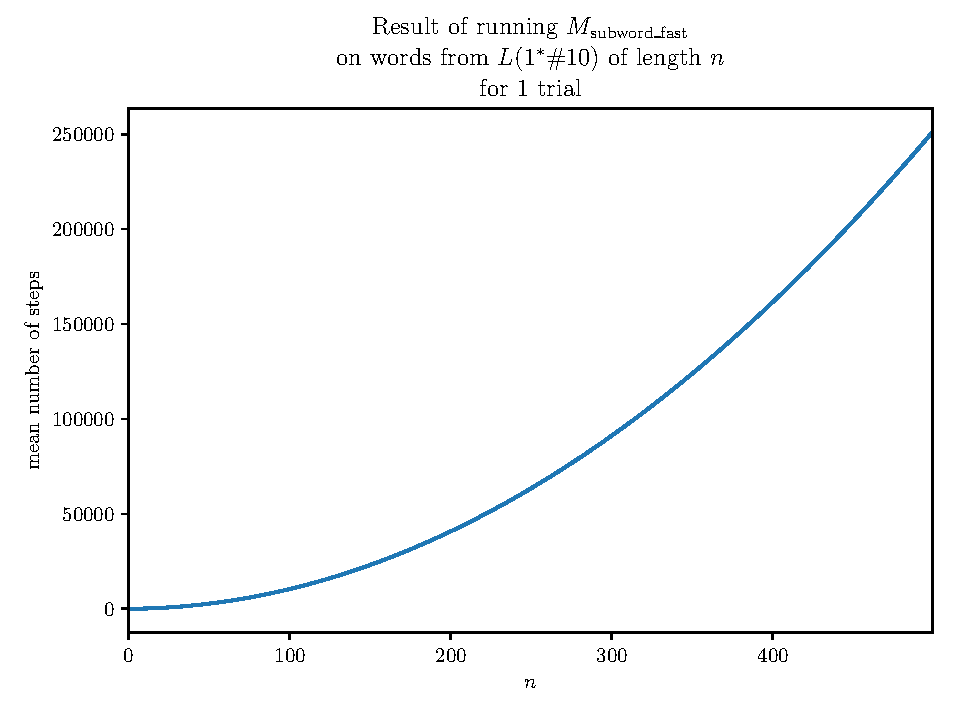
\includegraphics[width=\textwidth]{images/plots/subword_fast-ones.pdf}
\end{center}

Similarly, the other plots are available in section \ref{plots_subword_fast}, and the CSV data is in \code{data/subword\_fast-*.csv}. 